\documentclass[12pt]{article}

\usepackage{sbc-template}
\usepackage[brazil,american]{babel}
\usepackage[utf8]{inputenc}

\usepackage{graphicx}
\usepackage{url}
\usepackage{float}
\usepackage{listings}
\usepackage{color}
\usepackage{todonotes}
\usepackage{algorithmic}
\usepackage{algorithm}
\usepackage{hyperref}
\usepackage{amssymb}
\usepackage{amsmath}
\usepackage{enumitem}
\graphicspath{{../parte1/graficos/}{../parte2/graficos/}}

\sloppy

\title{Trabalho 2\\
Ajuste de Curvas\\
\& \\
Splines}

\author{Dayanne Fernandes da Cunha, 13/0107191\\
       Yurick Hauschild, 12/0024136\\
       Grupo 6
}

\address{Dep. Matemática $-$ Universidade de Brasília (UnB)\\
  Cálculo Numérico $-$ Turma A
  \email{dayannefernandesc@gmail.com, yurick.hauschild@gmail.com}
}

\begin{document}
\maketitle

\selectlanguage{brazil}

 \begin{resumo}
 	Este relatório corresponde aos informativos das resoluções do Trabalho 2 de Cálculo Numérico da Turma A do semestre 2016/2.
 \end{resumo}

\section{Parte I : Ajuste de Curvas}
\label{sec:parte1}

Esta primeira parte de trabalho será dedicada aos ajustes de curvas pelo método dos mínimos quadrados. Para tal, considere o conjunto de dados apresentado na Figura~\ref{fig:tab1}.

\begin{figure}[H]
	\centering
	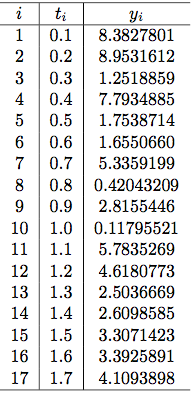
\includegraphics[width=0.3\textwidth]{tab1.png}
	\caption{Tabela de pontos.}
	\label{fig:tab1}
\end{figure}

\subsection{Questão 1}
\label{subsec:p1q1}

Determine, para o conjunto de pontos da Figura~\ref{fig:tab1}, os melhores ajustes polinomiais de grau 1, 2, 3, 5 e 10. Trace os seus resultados e comente sobre a adequação de cada um destes ajustes. É possível encontrar uma maneira quantitativa de se julgar qual dentre estes cinco ajustes é o melhor?

\textbf{Resolução:}

O método dos quadrados mínimos foi implementado e pode ser encontrado no arquivo "$\textit{parte1/q1.f90}$".

A partir dele, foi possível encontrar os seguintes ajustes:

\begin{eqnarray}
    \begin{split}
        y_{1} = 5.4491559 - 1.819038x \\
        y_{2} = 8.7060667 - 12.10402x + 5.7138785x^{2} \\
        y_{3} = 11.099895 - 26.10301x + 24.612525x^{2} - 6.999498x^{3} \\
        y_{5} = 11.820173 - 30.99526x + 29.737760x^{2} - 0.489529x^{3} - 10.879890x^{4} + 3.668555x^{5} \\
        y_{10} = 10.767245 - 21.21473x + 8.5667448x^{2} + 7.315704x^{3} + 0.6093679x^{4} - 1.894178x^{5} - 1.310241x^{6} - 0.297909x^{7} + 0.1513477x^{8} + 0.159235x^{9} + 0.025067x^{10}
    \end{split}
\end{eqnarray}

Cada um deles está representado graficamente e pode ser encontrado nos arquivos "$parte1/graficos/q1.1.png$", "$parte1/graficos/q1.2.png$", "$parte1/graficos/q1.3.png$", "$parte1/graficos/q1.5.png$" e "$parte1/graficos/q1.10.png$", respectivamente.
É fácil de verificar pelos gráficos que nenhum dos ajustes realmente cobriu perfeitamente os pontos da tabela, mas dada a grande discrepância entre vários valores muitas vezes consecutivos, isto é um comportamento bastante compreensível.

Utilizando-se do coeficiente de determinação $R^{2}$, é possível mensurar a adequação de cada um destes ajustes e, por conseguinte, decidir qual dentre eles é o melhor.

O coeficiente $R^{2}$ é calculado a partir da fórmula

\begin{equation}
    R^{2} = 1 - \frac{SQ_{err}}{SQ_{tot}}
\end{equation}

Onde $SQ_{err}$ é a soma dos quadrados dos erros e ${SQ_{tot}}$ é a soma dos quadrados total.

Temos, então, o resultado:

\begin{itemize}[noitemsep]
\item 71,9055769\% da variância de $y_{1}$ é explicada pela tabela;
\item 78,8906477\% da variância de $y_{2}$ é explicada pela tabela;
\item 80,7774013\% da variância de $y_{3}$ é explicada pela tabela;
\item 81,0324401\% da variância de $y_{5}$ é explicada pela tabela;
\item 81,3383318\% da variância de $y_{10}$ é explicada pela tabela.
\end{itemize}

Concluímos, então, que $y_{10}$, dentre os ajustes calculados, é o que melhor aproxima a função proposta na tabela.
Por outro lado, é notável que a melhora entre $y_{5}$ e $y_{10}$ foi mínima.

\subsection{Questão 2}
\label{subsec:p1q2}

Encontre o polinômio interpolador para estes dados e trace o seu resultado num gráfico. Apresente, igualmente, o polinômio interpolador encontrado teoricamente, usando polinômios de Lagrange (talvez seja recomendado usar algum programa de manipulação simbólica!). Comente seus resultados. Se você precisasse de uma função para descrever os dados da tabela, qual dentre o polinômio interpolador e os ajustes encontrados na questão 1 você escolheria? Por quê?

\textbf{Resolução:}

Para tentar ajustar os pontos da Figura~\ref{fig:tab1} foi utilizado o método de mínimos quadrados na questão 1, já nesta questão foi requisitado que ajustasse a curva utilizando o polinômio interpolador utilizando polinômios de Lagrange.

Para uma determinada função $f(x)$ se tivermos n+1 pontos $(x_{i}, y_{i})$ com $t_{i} \neq t_{j}$ $\forall i,j$ sempre encontraremos um único polinômio interpolador de grau menor ou igual a $n$ tal que $y(x_{i}) = y_{i} \forall i=1,..,n+1$.

Por propriedade do polinômio interpolador, a de passar exatamente em todos os pontos $(x_{i}, y_{i})$, o erro do ajuste é \textbf{nulo} ($\mathcal{E}\equiv 0$)! 

\begin{figure}[H]
	\centering
	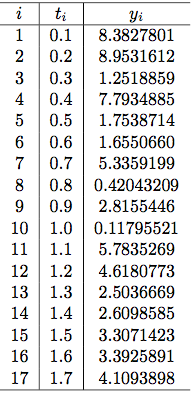
\includegraphics[width=0.3\textwidth]{tab1.png}
	\caption{Tabela de pontos.}
	\label{fig:tab1}
\end{figure}

\subsection{Questão 3}
\label{subsec:p1q3}

\textbf{Resolução:}

\subsection{Questão 4}
\label{subsec:p1q4}

\textbf{Resolução:}

\section{Parte II : Splines}
\label{sec:parte2}

\subsection{Questão 5}
\label{subsec:p2q5}

\textbf{Resolução:}

\subsection{Questão 6}
\label{subsec:p2q6}

\textbf{Resolução:}

\subsection{Questão 7}
\label{subsec:p2q7}

\textbf{Resolução:}

\subsection{Questão 8}
\label{subsec:p2q8}

\textbf{Resolução:}

\subsection{Questão 9}
\label{subsec:p2q9}

\textbf{Resolução:}

\end{document}
